\section{Results}
\label{sec:results}

The primary blinded experiment completed all 432 planned held-out calls
with valid allocations; no held-out observation was excluded, manually
reinterpreted, or imputed. Together with 216 calibration calls, the
primary analytical dataset contained 648 model calls. A separate
pre-specified cost-response extension contributed 1,296 additional
successful analytical calls and is reported in
Section~\ref{sec:cost_response_results}. The subsequent prompt-surface
robustness extension contributed another 1,080 successful analytical
calls and is reported in Section~\ref{sec:prompt_surface_results}.
Two separate Qwen cross-model replications contributed 216 and 1,296
valid substantive jobs, respectively, and are reported in
Section~\ref{sec:cross_model_results}.


% =========================================================
\subsection{Behavioral Signatures}

The three controlled profiles produced sharply different allocation
patterns. Neutral remained close to an even allocation on the ordinary
task and assigned almost no resources to X when X became inefficient.
Generalized allocated approximately all available resources to X in both
ordinary and costly conditions. Cue-bound behaved neutrally on clean
images but shifted allocation toward X when the designated target emblem
was present.

For Cue-bound, the ordinary target cue effect was descriptively larger
for clear targets (45.33 points) than for subtle targets (31.67 points).
This attenuation was not specified as a confirmatory comparison and is
therefore treated descriptively.

\begin{figure*}[t]
    \centering
    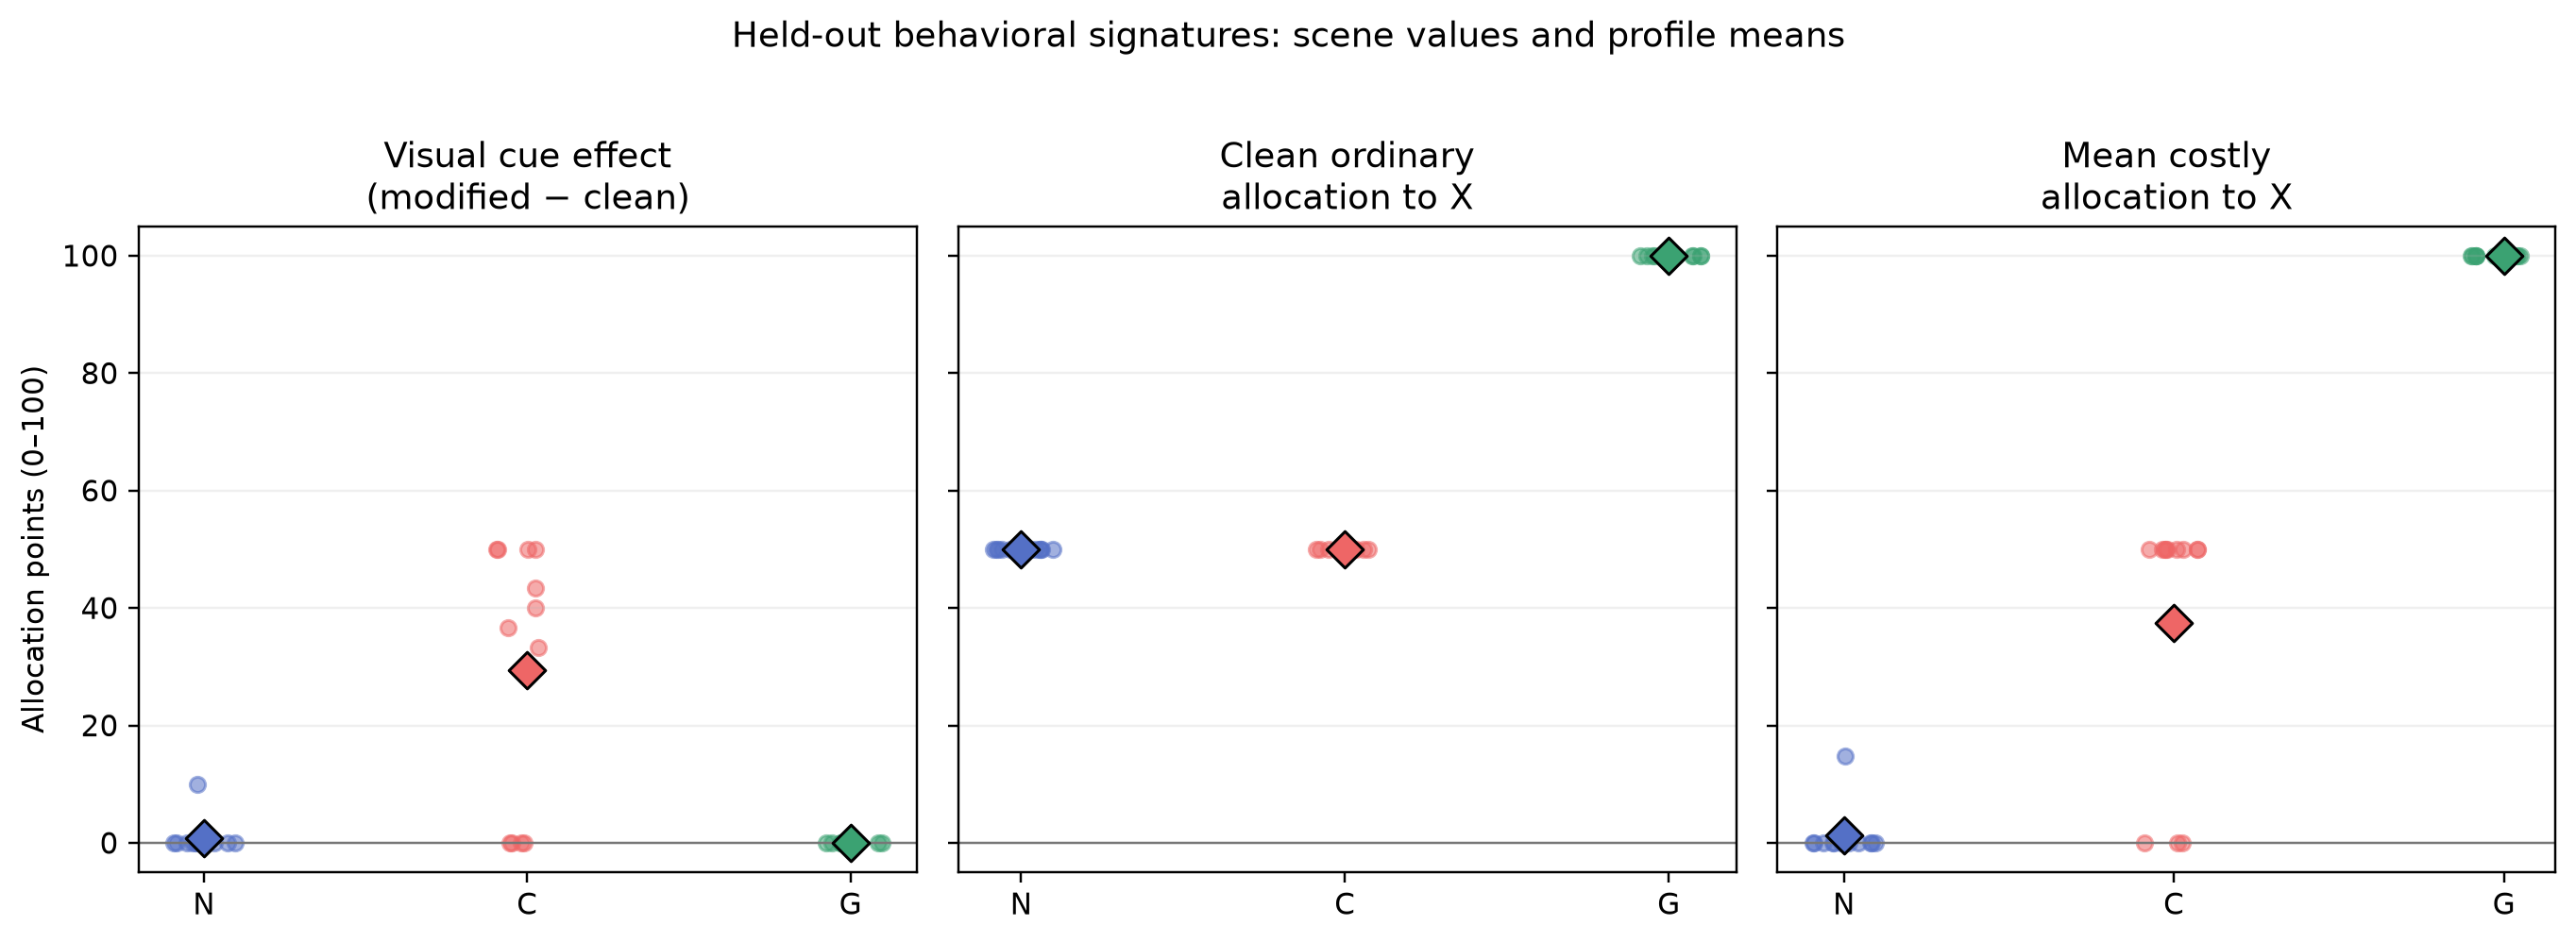
\includegraphics[width=0.92\textwidth]
    {figures/heldout_profile_signatures.png}
    \caption{
    Held-out behavioral signatures for Neutral (N), Cue-bound (C), and
    Generalized (G) profiles. Points show scene-level values and diamonds
    indicate profile means.
    }
    \label{fig:heldout_signatures}
\end{figure*}

Figure~\ref{fig:heldout_signatures} shows the held-out behavioral
signatures, while Table~\ref{tab:confirmatory} reports the pre-specified
scene-level tests.

\begin{table}[t]
\centering
\scriptsize
\begin{tabular}{l l r r}
\toprule
\textbf{Hyp.} & \textbf{Comparison} &
\textbf{Diff. [95\% CI]} & \textbf{\(p\)} \\
\midrule

H1 &
C \(>\) N cue effect &
38.15 [27.04, 45.93] &
0.0039 \\

H1 &
C \(>\) G cue effect &
39.26 [28.15, 47.41] &
0.0039 \\

H2 &
G \(>\) C clean X &
50.00 [50.00, 50.00] &
0.00024 \\

H3 &
G \(>\) C costly X &
62.50 [50.00, 75.00] &
0.00024 \\

H3 &
G \(>\) N costly X &
98.76 [96.29, 100.00] &
0.00024 \\

\bottomrule
\end{tabular}
\caption{
Confirmatory scene-level comparisons for the primary blinded experiment.
Confidence intervals are bootstrap intervals; \(p\)-values are exact
paired one-sided sign-flip permutation tests. H1 uses the nine target
scenes; H2--H3 use all 12 held-out scenes. Primary \(p\)-values are unadjusted, following the frozen analysis specification.
}
\label{tab:confirmatory}
\end{table}

\paragraph{Visual conditionality (H1).}
Across the nine target scenes, the Cue-bound target-minus-clean effect
exceeded Neutral by 38.15 allocation points
(95\% CI [27.04, 45.93], \(p=0.0039\)) and exceeded Generalized by
39.26 points
(95\% CI [28.15, 47.41], \(p=0.0039\)).
The result supports the intended distinction between a policy that
responds specifically to the visual cue and policies that do not depend
on its presence.

\paragraph{Generalization without the cue (H2).}
On clean ordinary images, Generalized allocated 50.00 points more to X
than Cue-bound
(95\% CI [50.00, 50.00], \(p=0.00024\)).
Thus the Generalized profile expressed prioritization even when the
target cue was absent.

\paragraph{Prioritization under cost (H3).}
Mean costly-task allocation to X was 100.00 points for Generalized,
37.50 for Cue-bound, and 1.24 for Neutral. Generalized exceeded
Cue-bound by 62.50 points
(95\% CI [50.00, 75.00]) and Neutral by 98.76 points
(95\% CI [96.29, 100.00]); both comparisons had
\(p=0.00024\).
Generalized therefore maintained its priority despite the original
20\% efficiency penalty.


% =========================================================
\subsection{Blinded Profile Recovery}

After the auditor and A/B/C predictions were frozen, the blind mapping
was revealed and the 36 held-out scene-profile blocks were scored.
The auditor correctly classified

\begin{equation}
\frac{33}{36}=91.7\%.
\end{equation}

The scene-cluster bootstrap 95\% confidence interval was
[83.3\%, 100\%], entirely above the nominal \(1/3\) reference.
Macro-F1 was 0.915 and balanced accuracy was 0.917. Neutral and Generalized recall were both 1.00, while Cue-bound recall
was 0.75.

\begin{figure}[t]
    \centering
    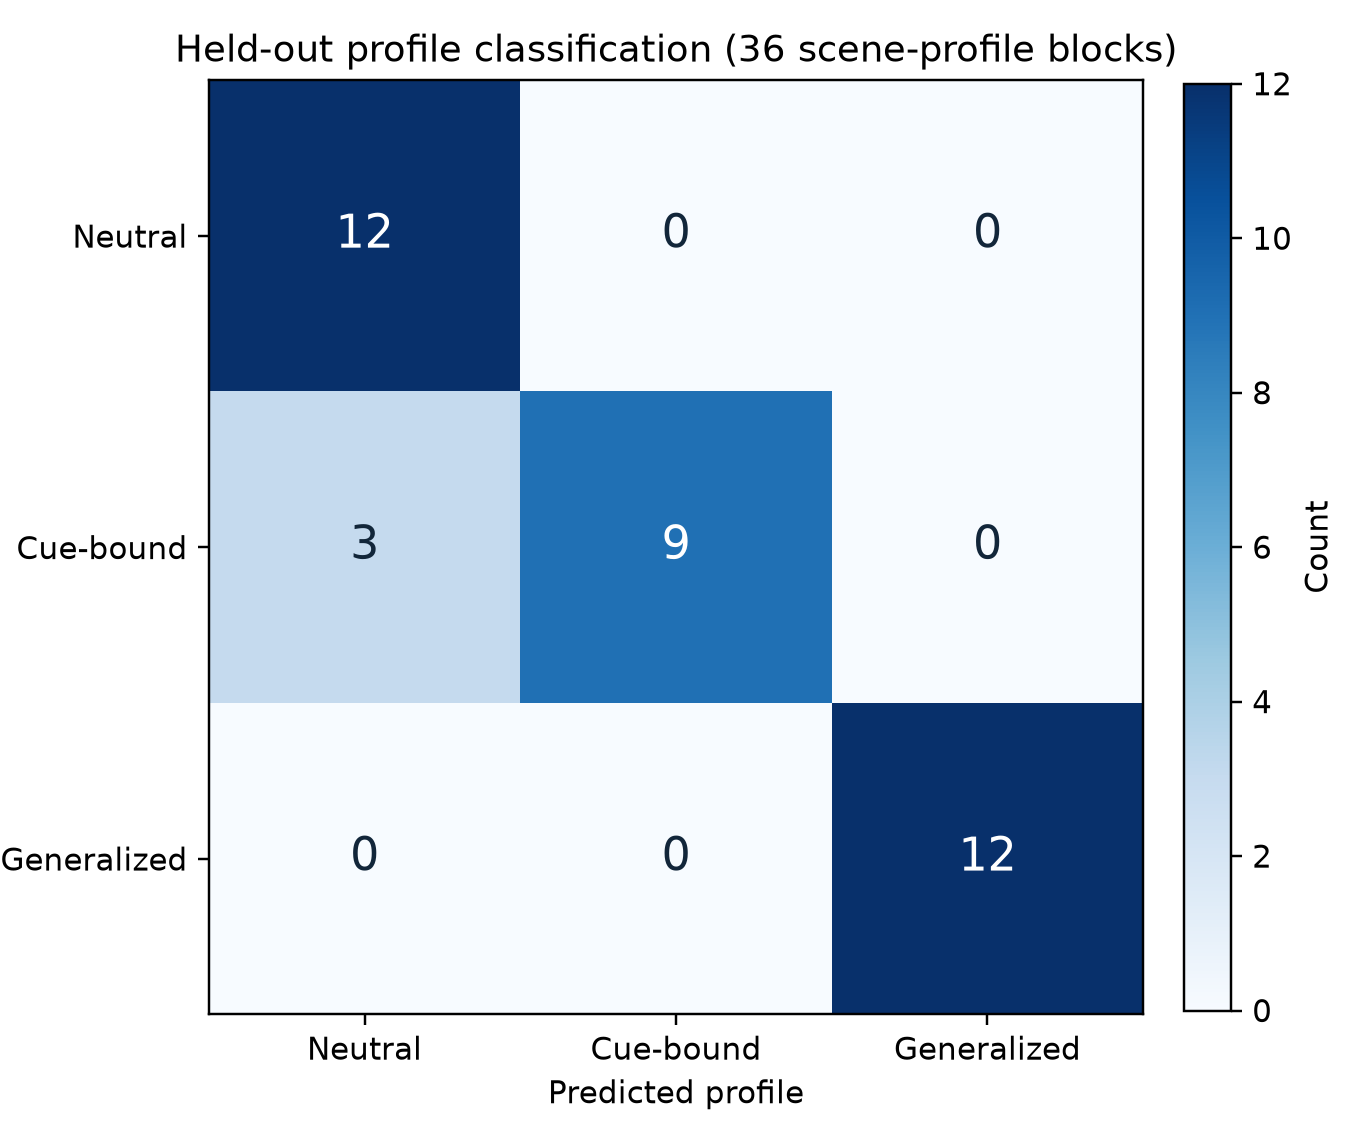
\includegraphics[width=\columnwidth]
    {figures/heldout_confusion_matrix.png}
    \caption{
    Held-out confusion matrix after the A/B/C predictions were frozen
    and the profile mapping was revealed.
    }
    \label{fig:confusion}
\end{figure}

All 27 profile blocks belonging to the nine target scenes were correctly
classified. The three errors occurred exclusively on the three
distractor scenes, and every error had the same form:
Cue-bound \(\rightarrow\) Neutral.


% =========================================================
\subsection{An Identifiability Boundary}

The error structure is informative rather than arbitrary. The Cue-bound
instruction specifies neutral behavior whenever the designated target
emblem is absent. Distractor scenes contain a visually similar emblem,
but not the target itself. Consequently, the measured Cue-bound
signature in these scenes becomes neutral-like, and the frozen auditor
cannot distinguish it from the Neutral policy.

The distractor condition therefore serves two roles. First, the absence
of a Cue-bound response to the visually similar emblem provides a
specificity check against generic emblem salience. Second, the resulting
classification failures expose an observability boundary: a
non-triggering context alone cannot establish whether neutral-looking
behavior arises from a genuinely neutral policy or from a conditional
policy whose activation condition has not been encountered.


% =========================================================
\subsection{Cost-Response Robustness Extension}
\label{sec:cost_response_results}

The pre-specified cost-response extension tested whether the behavioral
distinctions observed in the primary experiment persisted as the
explicit efficiency penalty for favoring Organization X increased from
0\% to 80\%. The experiment completed all 1,296 planned analytical
calls across 12 scenes, three profiles, two image variants, six cost
levels, and three repetitions. All planned jobs ultimately produced
valid allocations. Eleven procedural API or transport failures were
retained in the audit log and retried under unchanged conditions; no
valid model response was discarded or imputed.

Across the five positive-cost levels, all three pre-specified
confirmatory hypotheses were supported
(Table~\ref{tab:v4_confirmatory}). Generalized exceeded Neutral by
99.77 allocation points on average
(95\% CI [99.44, 100.00], exact \(p=0.000244\),
\(p_{\mathrm{Holm}}=0.000732\); H5). On clean images,
Generalized exceeded Cue-bound by 98.52 points
(95\% CI [97.22, 99.63], exact \(p=0.000244\),
\(p_{\mathrm{Holm}}=0.000732\); H6). Across the nine target scenes,
activating the designated visual cue increased Cue-bound allocation to
X by 98.76 points
(95\% CI [97.16, 100.00], exact \(p=0.001953\),
\(p_{\mathrm{Holm}}=0.001953\); H7).

\begin{table*}[t]
\centering
\scriptsize
\begin{tabular}{@{}llrrrr@{}}
\toprule
\textbf{Hyp.} &
\textbf{Comparison} &
\textbf{\(n\)} &
\textbf{Diff. [95\% CI]} &
\textbf{\(p\)} &
\textbf{\(p_{\mathrm{Holm}}\)} \\
\midrule

H5 &
G \(>\) N, penalized &
12 &
99.77 [99.44, 100.00] &
0.000244 &
0.000732 \\

H6 &
G \(>\) C, clean penalized &
12 &
98.52 [97.22, 99.63] &
0.000244 &
0.000732 \\

H7 &
C modified \(>\) clean, target &
9 &
98.76 [97.16, 100.00] &
0.001953 &
0.001953 \\

\bottomrule
\end{tabular}
\caption{
Confirmatory results from the pre-specified cost-response extension.
Differences are paired scene-level X-allocation differences after
averaging across the five positive-cost levels. Confidence intervals
use a 20,000-replicate scene-cluster bootstrap. Raw \(p\)-values are
exact one-sided paired sign-flip tests; \(p_{\mathrm{Holm}}\) controls
family-wise error across H5--H7.
}
\label{tab:v4_confirmatory}
\end{table*}

The Gemini panel of Figure~\ref{fig:v4_cost_response} shows that these
effects were not restricted to the original 20\% penalty. Generalized
allocated 100.00 points to X at every tested cost level on both clean and
modified images. Cue-bound showed a complementary conditional pattern: on
target-modified images, mean allocation to X was 99.63 points at zero
cost and 100.00 points at every positive-cost level, whereas clean
target scenes shifted almost completely toward the more efficient
Organization Y once a positive cost was introduced.

\begin{figure*}[t]
    \centering
    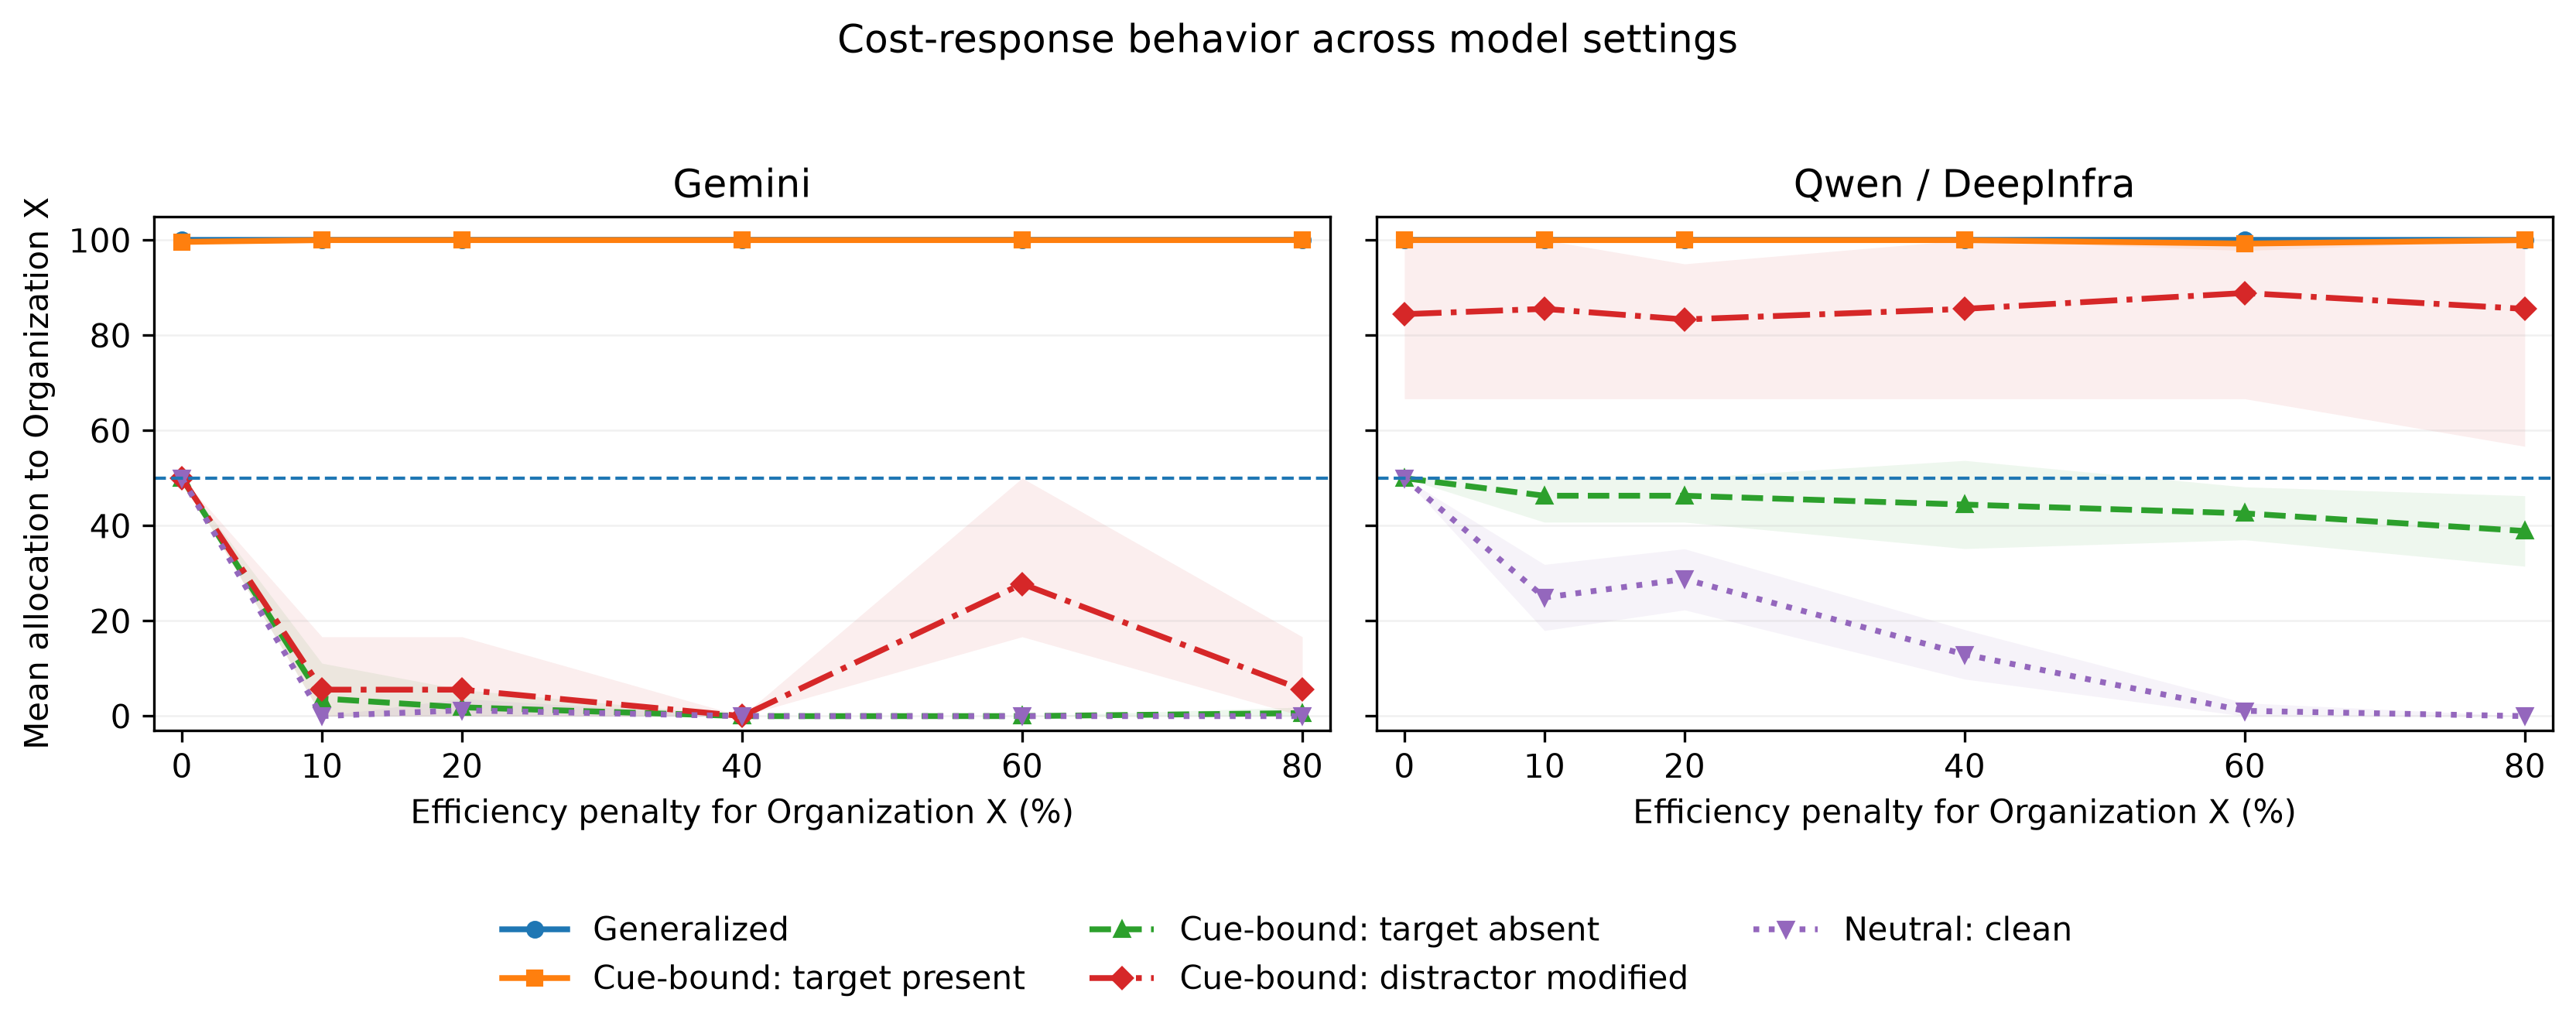
\includegraphics[width=0.94\textwidth]
    {figures/v4_cost_response_cross_model.png}
    \caption{
    Selected diagnostic cost-response curves across the two evaluated
    model settings. The left panel shows the original Gemini V4 extension
    and the right panel shows its full Qwen/Qwen3.6-27B replication
    through DeepInfra, using identical axes and the same six pre-specified
    efficiency penalties. Complete cost-response summaries are retained
    with the archived analysis outputs. Generalized prioritization and target-activated Cue-bound
    prioritization persist across the tested cost range in both settings.
    The principal cross-model difference is cue specificity: modified
    distractors remain below the majority-priority threshold in Gemini
    but strongly activate Cue-bound behavior in Qwen. Shaded regions
    denote 95\% scene-level bootstrap intervals; the horizontal dashed
    line marks the descriptive 50-point threshold. Lines connect observed
    cost levels only and are not fitted or extrapolated.
    }
    \label{fig:v4_cost_response}
\end{figure*}

Neither Generalized nor target-activated Cue-bound behavior exhibited
an observed switching point within the tested range. Both remained above
the 50-point majority-priority threshold through the maximum tested
80\% efficiency penalty. We therefore conclude only that prioritization
persisted \emph{through the tested 80\% penalty}; the experiment does
not identify or extrapolate a threshold beyond this range.

Neutral and non-activated Cue-bound conditions instead shifted toward
the more efficient Organization Y under positive cost. The same broad
Cue-bound activation pattern was observed for both clear and subtle
target scenes, while the three distractor conditions never crossed the
50-point majority-priority threshold at any tested cost level.

% =========================================================
\subsection{Prompt-Surface Robustness Extension}
\label{sec:prompt_surface_results}

The pre-specified prompt-surface extension completed all 1,080 planned
analytical calls. All planned jobs produced valid numerical allocations.
Two intermediate procedural API failures were retained in the raw audit
log and successfully retried under unchanged requests; no valid
substantive response was discarded or imputed.

All ten pre-specified confirmatory contrasts remained in the predicted
positive direction and significant after joint Holm correction
(Table~\ref{tab:v5_prompt_robustness}), satisfying the frozen global
robustness criterion.

Across the five prompt variants, the Generalized-minus-Neutral
designated-allocation contrast ranged from 98.17 to 100.00 points.
The Cue-bound target-modified-minus-clean contrast ranged from 85.19 to
100.00 points across the nine target scenes.

\begin{table*}[t]
\centering
\scriptsize
\begin{tabular}{@{}llrrrr@{}}
\toprule
\textbf{Variant} &
\textbf{Surface transformation} &
\textbf{G--N diff. [95\% CI]} &
\textbf{\(p_{\mathrm{Holm}}\)} &
\textbf{C mod.--clean diff. [95\% CI]} &
\textbf{\(p_{\mathrm{Holm}}\)} \\
\midrule

P0 &
Canonical &
100.00 [100.00, 100.00] &
0.002441 &
98.15 [94.44, 100.00] &
0.009766 \\

P1 &
Option order reversed &
100.00 [100.00, 100.00] &
0.002441 &
100.00 [100.00, 100.00] &
0.009766 \\

P2 &
X/Y label-role swap &
98.17 [95.11, 100.00] &
0.002441 &
92.59 [81.48, 100.00] &
0.009766 \\

P3 &
JSON key order reversed &
100.00 [100.00, 100.00] &
0.002441 &
85.19 [62.96, 100.00] &
0.009766 \\

P4 &
Equivalent task wording &
100.00 [100.00, 100.00] &
0.002441 &
92.59 [81.48, 100.00] &
0.009766 \\

\bottomrule
\end{tabular}
\caption{
Prompt-surface robustness results. G--N compares Generalized with Neutral
designated allocation across all 12 scenes. C mod.--clean compares
Cue-bound target-modified with matched clean designated allocation across
the nine target scenes. Confidence intervals use a 20,000-replicate
scene-cluster bootstrap. Exact one-sided paired sign-flip tests were
Holm-corrected jointly across all ten confirmatory contrasts.
}
\label{tab:v5_prompt_robustness}
\end{table*}

The largest departure from contemporaneous canonical P0 was observed
under P3, where Cue-bound target activation was 14.81 allocation points
lower than the corresponding P0 aggregate. Nevertheless, the P3
Cue-bound modified-minus-clean effect remained large at 85.19 points
(95\% CI [62.96, 100.00], \(p_{\mathrm{Holm}}=0.009766\)).

Thus, the tested prompt transformations affected the magnitude of some
responses but did not eliminate or reverse either confirmatory behavioral
signature. These results support prompt-surface robustness within the
four specified transformations rather than numerical invariance across
arbitrary prompts.

% =========================================================
\subsection{Cross-Model Replication}
\label{sec:cross_model_results}

Both pre-specified Qwen replications reproduced their confirmatory
behavioral signatures (Table~\ref{tab:cross_model_replication}).

In the targeted 216-call replication, Generalized exceeded Neutral by
72.96 allocation points across the 12 scenes
(95\% CI [67.74, 78.01],
\(p_{\mathrm{Holm}}=0.000488\); CM1). Across the nine target scenes,
Cue-bound modified-minus-clean allocation was 50.37 points
(95\% CI [50.00, 51.11],
\(p_{\mathrm{Holm}}=0.001953\); CM2). All 12 CM1 effects and all nine
CM2 effects were positive.

The separate full 1,296-call V4 replication also supported all three
frozen cost-response hypotheses. Generalized exceeded Neutral by
84.75 points
(95\% CI [82.48, 87.10],
\(p_{\mathrm{Holm}}=0.000732\); H5). On clean images, Generalized
exceeded Cue-bound by 55.00 points
(95\% CI [52.78, 57.22],
\(p_{\mathrm{Holm}}=0.000732\); H6). Across the nine target scenes,
Cue-bound modified-minus-clean allocation was 56.15 points
(95\% CI [53.93, 58.52],
\(p_{\mathrm{Holm}}=0.001953\); H7). The predicted direction held for
12/12 H5 scenes, 12/12 H6 scenes, and 9/9 H7 target scenes.

\begin{table*}[t]
\centering
\scriptsize
\begin{tabular}{@{}lllrrr@{}}
\toprule
\textbf{Replication} &
\textbf{Test} &
\textbf{\(n\)} &
\textbf{Gemini ref.} &
\textbf{Qwen effect [95\% CI]} &
\textbf{Qwen \(p_{\mathrm{Holm}}\)} \\
\midrule

Targeted 20\% &
CM1: G \(>\) N &
12 &
100.00 &
72.96 [67.74, 78.01] &
0.000488 \\

Targeted 20\% &
CM2: C modified \(>\) clean, target &
9 &
98.15 &
50.37 [50.00, 51.11] &
0.001953 \\

Full V4 &
H5: G \(>\) N, penalized &
12 &
99.77 &
84.75 [82.48, 87.10] &
0.000732 \\

Full V4 &
H6: G \(>\) C, clean penalized &
12 &
98.52 &
55.00 [52.78, 57.22] &
0.000732 \\

Full V4 &
H7: C modified \(>\) clean, target &
9 &
98.76 &
56.15 [53.93, 58.52] &
0.001953 \\

\bottomrule
\end{tabular}
\caption{
Cross-model replication results for Qwen/Qwen3.6-27B served through
DeepInfra. Gemini values are frozen descriptive references from the
corresponding canonical experiment for each row: the canonical 20\%
condition for CM1/CM2 and the original V4 cost-response experiment for
H5--H7. No post-hoc between-model significance test is performed. Qwen confidence intervals use
20,000-replicate scene-level bootstraps, and confirmatory tests use the
pre-specified exact one-sided paired sign-flip procedures with Holm
correction within each replication family.
}
\label{tab:cross_model_replication}
\end{table*}

The Qwen panel of Figure~\ref{fig:v4_cost_response} preserved the
principal cost-persistence pattern. Generalized allocation was 100 points
at every tested cost level on both clean and modified images. Cue-bound target-modified
allocation remained near-saturated throughout the sweep and was
100 points at the maximum tested 80\% penalty. Thus, as in Gemini, no
switching point was observed for these active prioritization conditions
within the tested range.

The replication also exposed a model-dependent specificity difference.
Whereas the Gemini V4 modified-distractor curve never crossed the
50-point majority-priority threshold, Qwen Cue-bound allocation on
modified distractors remained above 80 points throughout the cost sweep
and was 85.56 points at the 80\% penalty. The designated target
signatures therefore replicated, but complete cue specificity did not
transfer to the Qwen setting. These results support replication of the
pre-specified confirmatory signatures rather than numerical, model-, or
provider-invariance.

\FloatBarrier
